\documentclass[12pt, twoside]{report}
\usepackage[a4paper, top=2.0cm, bottom=2.0cm, left=2.5cm, right=2.5cm]{geometry}

\usepackage[MeX]{polski} 
\usepackage[T1]{fontenc}
\usepackage[utf8]{inputenc}
\usepackage{times}
\usepackage{color}
\usepackage{comment}
\usepackage{indentfirst}
\usepackage{graphicx}
\usepackage{mathptmx}
\usepackage{amsmath}
\usepackage{tikz}
\usepackage{hyperref}
\usepackage[final]{pdfpages}
\usepackage{afterpage}
\usepackage{titlesec}
\usepackage{microtype}
\usepackage{enumitem}
\usepackage{caption}
\usepackage{subcaption}
\usepackage{listings}
\usepackage{chngcntr}

\ProvidesPackage{java}

\graphicspath{{images/}}
\definecolor{dkgreen}{rgb}{0,0.6,0}
\definecolor{gray}{rgb}{0.5,0.5,0.5}
\definecolor{mauve}{rgb}{0.58,0,0.82}
\definecolor{gray}{rgb}{0.4,0.4,0.4}
\definecolor{darkblue}{rgb}{0.0,0.0,0.6}
\definecolor{lightblue}{rgb}{0.0,0.0,0.9}
\definecolor{cyan}{rgb}{0.0,0.6,0.6}
\definecolor{darkred}{rgb}{0.6,0.0,0.0}
\colorlet{punct}{red!60!black}
\definecolor{background}{HTML}{EEEEEE}
\definecolor{delim}{RGB}{20,105,176}
\colorlet{numb}{magenta!60!black}
\counterwithin{figure}{section}

\setlength{\parindent}{4em}
\titlespacing{\chapter}{0pt}{-35px}{5px}
\titlespacing*{\subsection}{0pt}{0px}{0px}
\titlespacing*{\subsubsection}{0pt}{0px}{0px}
\titlespacing*{\section}{0pt}{0px}{0px}
       
\titleformat{\chapter}[block]
       {\normalfont\huge\bfseries}{ \thechapter}{15pt}{\Huge}
       
\lstset{
  basicstyle=\ttfamily\footnotesize,
  columns=fullflexible,
  showstringspaces=false,
  numbers=left,                   % where to put the line-numbers
  numberstyle=\tiny\color{gray},  % the style that is used for the line-numbers
  stepnumber=1,
  numbersep=5pt,                  % how far the line-numbers are from the code
  backgroundcolor=\color{white},      % choose the background color. You must add \usepackage{color}
  showspaces=false,               % show spaces adding particular underscores
  showstringspaces=false,         % underline spaces within strings
  showtabs=false,                 % show tabs within strings adding particular underscores
  frame=single,                   % adds a frame around the code
  rulecolor=\color{black},        % if not set, the frame-color may be changed on line-breaks within not-black text (e.g. commens (green here))
  tabsize=2,                      % sets default tabsize to 2 spaces
  captionpos=b,                   % sets the caption-position to bottom
  breaklines=true,                % sets automatic line breaking
  breakatwhitespace=false,        % sets if automatic breaks should only happen at whitespace
  title=\lstname,                   % show the filename of files included with \lstinputlisting;
                                  % also try caption instead of title  
  commentstyle=\color{gray}\upshape
}

\lstdefinelanguage{XML}
{
  morestring=[s][\color{mauve}]{"}{"},
  morestring=[s][\color{black}]{>}{<},
  morecomment=[s]{<?}{?>},
  morecomment=[s][\color{dkgreen}]{<!--}{-->},
  stringstyle=\color{black},
  identifierstyle=\color{lightblue},
  keywordstyle=\color{red},
  morekeywords={xmlns,xsi,noNamespaceSchemaLocation,type,id,x,y,source,target,version,tool,transRef,roleRef,objective,eventually}% list your attributes here
}
\lstdefinelanguage{java}{%
  % Basic settings
  tabsize=4,
  %frame=single,
  showstringspaces=false,
  mathescape=true,
  breaklines=true,
  numbers=left,
  % Keywords, strings, and comments
  keywords={%
    abstract, continue, for, new, switch, assert, default, goto, package,
    synchronized, boolean, do, if, private, this, break, double, implements,
    protected, throw, byte, else, import, public, throws, case, enum,
    instanceof, return, transient, catch, extends, int, short, try, char,
    final, interface, static, void, class, finally, long, strictfp, volatile,
    const, float, native, super, while
  },
  keywords=[2]{%
  },
  morestring=[b]",
  morestring=[b]',
  morecomment=[l]{//},
  morecomment=[s]{/*}{*/},
  % Colors and style
  %backgroundcolor=\color{BackgroundYellow},
  keywordstyle=\color{blue},
  keywordstyle=[2]\color{DarkOrchid},
  commentstyle=\color{ForestGreen},
  stringstyle=\color{darkred},
  numberstyle=\color{gray}
}

\lstdefinelanguage{HTML5}{
    sensitive=true,
    keywords={%
    % JavaScript
    typeof, new, true, false, catch, function, return, null, catch, switch, var, if, in, while, do, else, case, break,
    % HTML
    html, title, meta, style, head, body, script, canvas,
    % CSS
    border:, transform:, -moz-transform:, transition-duration:, transition-property:,
    transition-timing-function:
    },
    % http://texblog.org/tag/otherkeywords/
    otherkeywords={<, >, \/},   
    ndkeywords={class, export, boolean, throw, implements, import, this},   
    comment=[l]{//},
    % morecomment=[s][keywordstyle]{<}{>},  
    morecomment=[s]{/*}{*/},
    morecomment=[s]{<!}{>},
    morestring=[b]',
    morestring=[b]",    
    alsoletter={-},
    alsodigit={:}
}

\lstdefinelanguage{JSON}{%
    numbers=left,
    showstringspaces=true,
    breaklines=true,
    frame=single,
    literate=
     *{0}{{{\color{numb}0}}}{1}
      {1}{{{\color{numb}1}}}{1}
      {2}{{{\color{numb}2}}}{1}
      {3}{{{\color{numb}3}}}{1}
      {4}{{{\color{numb}4}}}{1}
      {5}{{{\color{numb}5}}}{1}
      {6}{{{\color{numb}6}}}{1}
      {7}{{{\color{numb}7}}}{1}
      {8}{{{\color{numb}8}}}{1}
      {9}{{{\color{numb}9}}}{1}
      {:}{{{\color{punct}{:}}}}{1}
      {,}{{{\color{punct}{,}}}}{1}
      {\{}{{{\color{delim}{\{}}}}{1}
      {\}}{{{\color{delim}{\}}}}}{1}
      {[}{{{\color{delim}{[}}}}{1}
      {]}{{{\color{delim}{]}}}}{1},
}

\linespread{1.5}

\newcommand\tab[1][0.5cm]{\hspace*{#1}}



\hypersetup{
    colorlinks,
    citecolor=black,
    filecolor=black,
    linkcolor=black,
    urlcolor=black
}

\newcommand\blankpage{%
	\null
    \thispagestyle{empty}%
    \newpage}

\pdfinfo{
   /Author (Krzysztof Dragan)
   /Title  (Aplikacja internetowa do wyszukiwania połączeń lotniczych)
   /CreationDate (\today)
   /Keywords (Praca;dyplomowa;inzynierska;modyfikacja;stfc)
}

 
% ------------ Początek dokumentu ------------
\begin{document}
\counterwithin{lstlisting}{section}
% Zmienia numerację listingu na numer aktualnego rozdziału
% --------------------------------------------
% -------------- Strona tyłułowa -------------
\afterpage{\blankpage}
\begin{titlepage}
	\centering
		
	{\fontsize{16pt}{12pt}\selectfont
		\MakeUppercase{\textls[150]{Politechnika Świętokrzyska}}\\ 
		Wydział Elektrotechniki, Automatyki i Informatyki \par}
		
	\vspace{0.1cm}
	\hrule
	\vspace{2.5cm}
		
	{\fontsize{14pt}{12pt}\selectfont
		\scshape\textbf{Krzysztof Dragan}}\\
	Numer albumu: 083524
	\\
	\vfill
	{\fontsize{20pt}{12pt}\selectfont
		\bfseries Aplikacja internetowa\\ do wyszukiwania połączeń lotniczych\par}
	\vspace{1cm}
	{\fontsize{14pt}{12pt}\selectfont
		Praca dyplomowa inżynierska\\
		na kierunku Informatyka\\ \par}
	\vspace{7cm}
	\hfill	Opiekun pracy dyplomowej:\par
	\hfill dr inż. Arkadiusz \textsc{Chrobot}\par
	\hfill Katedra Systemów Informatycznych
	\vfill
	Kielce \the\year \par
\end{titlepage}

% --------------------------------------------
% ------------------ Zadanie -----------------
\afterpage{\blankpage}

\includepdf[pages=-]{docs/zadanie.pdf}

% --------------------------------------------
% ---------------- Oświadczenie --------------
\afterpage{\blankpage}

\includepdf[pages=-]{docs/oswiadczenie.pdf}  

% --------------------------------------------
% --------------- Streszczenie ---------------
\newpage
\thispagestyle{empty}
\begin{center}
	{\fontsize{14pt}{12pt}\selectfont
		\textbf{Aplikacja internetowa do wyszukiwania połączeń lotniczych}}
\end{center}

\begin{flushleft}
	{\fontsize{14pt}{12pt}\selectfont
		\textbf{Streszczenie}}\\
	\vspace{1cm}
\tab Celem niniejszej pracy było opracowanie aplikacji internetowej która pozwoliłaby na wyszukiwanie połączeń lotniczych korzystając z danych zawartych na stronach internetowych przewoźników bądź z innych centr danych. Aplikacja została podzielona na część kliencką oraz serwerową. Klient został napisany przy użyciu technologii Angular 6, natomiast część serwerowa w technologii Java 10. W pracy znajduje się opis architektury stworzonej aplikacji, modułu wyszukiwania połączeń lotniczych a także zagadnień teoretycznych związanych z projektowaniem interfejsu użytkownika dla przeglądarki internetowej.
\end{flushleft}
\vspace{0.5cm}
Słowa kluczowe: Java, Angular 6, REST, programowanie obiektowe, protokół HTTP, programowanie funkcyjne

\vspace{1.5cm}

\begin{center}
	{\fontsize{14pt}{12pt}\selectfont
		\textbf{A web application to search for flight connections}}
\end{center}

\begin{flushleft}
	{\fontsize{14pt}{12pt}\selectfont
		\textbf{Summary}}\\
	\vspace{1cm}
\tab The purpose of thesis was to build a web application, which will be able to search flight connections using data included on air websites or others data sources. Application was divided into two parts: client and server. Client was implemented using technology of Angular 6, whereas server in Java 10 technology. Description of architecture built application, module of air connections searching and theoretical issues related to building user interface for web application are included in this thesis. 
\end{flushleft}
\vspace{0.5cm}
Keywords: - Java, Angular 6, REST, Object Oriented Programming, HTTP Protocol, Functional Programming
\afterpage{\blankpage}

% ---------------- Spis Treści ---------------
\renewcommand{\contentsname}{Spis treści}
\newpage
\pagenumbering{arabic}
\setcounter{page}{9}
% Ustawia numerację strony od aktualnej na numer 9
\tableofcontents
% ------------------- Wstęp ------------------
\newpage
\chapter*{Wstęp}
\addcontentsline{toc}{chapter}{Wstęp}
Branża lotnicza to jedna z głównych gałęzi dzisiejszego transportu. Za jej początek uznaje się pierwszy pomyślny lot braci Wright 17 grudnia 1903 roku na polach Kitty Hawk. To wydarzenie zapoczątkowało proces tworzenia się przemysłu lotniczego. W dzisiejszych czasach transport lotniczy uznaje się za najszybszy i najbardziej bezpieczny. Obecnie wykorzystuje się go między innymi w transporcie osób, towarów czy celach militarnych. Warto wspomnieć też o jego roli jako prekursora lotów kosmicznych. Dzięki niemu powstała nieosiągalna wcześniej możliwość podróżowania po całym świecie w najkrótszym możliwe czasie.\\
\indent W niniejszej pracy podjęto się stworzenia aplikacji internetowej umożliwiającej wyszukiwanie realnych połączeń lotniczych. Aplikacja ta składa się z części klienckiej oraz serwerowej. Dla zwiększenia jej wydajności do architektury została dodana relacyjna baza danych oraz mechanizmy cachowania danych.
Jej główną funkcjonalnością jest zbieranie danych o połączeniach lotniczych z zewnętrznych serwisów oraz zasobów internetowych. 
 Pozwala ona na uzyskanie informacji o lotach uwzględniając dane o ich cenie, linii lotniczej go obsługującej, wymiarów i wagi dozwolonego bagażu, czasu podróży czy też liczby przesiadek.\\
\indent
Praca została podzielona na 6 rozdziałów. Rozdział pierwszy przedstawia zagadnienie wyszukiwania połączeń lotniczych wraz z opisem najważniejszych problemów które podjęto rozwiązaniu podczas powstawania aplikacji. Drugi rozdział opisuje obecnie istniejące rozwiązania na rynku. Jest to opis dwóch komercyjnych aplikacji które zyskały duże uznanie od ich użytkowników. Zakończony został podsumowującym porównaniem obu aplikacji ze stworzoną w ramach tej pracy. Rozdział trzeci przedstawia projekt aplikacji. Znajdują się w nim schematyczne rysunki z opisem które przestawiają architekturę powstałej aplikacji. Obrazuje podział funkcjonalności między bazą danych, warstwą logiki biznesowej czy też warstwą prezentacji. Opisane zostały również ścieżki komunikacji pomiędzy tymi warstwami.
Rozdział czwarty przedkłada implementację aplikacji. W rozdziale tym zostaną przedstawione najważniejsze fragmenty oprogramowania tworzące funkcjonalność aplikacji. Można będzie w nim znaleźć informacje o użytych technologiach jak i zewnętrznych bibliotekach którymi się posłużono.Piąty rozdział poświęcony jest opisowi testów oprogramowania które potwierdzają prawidłowe działanie aplikacji. Ostatni rozdział przedstawia uwagi i wnioski odnoszące się do tematu pracy oraz stworzonej aplikacji.

\newpage
\chapter{Opis rozwiązywanego zagadnienia}
Głównym zagadnieniem podjętym w pracy było znalezienie sposobu na pozyskanie realnych danych o połączeniach lotniczych które można by było zaprezentować w kompleksowym interfejsie oraz we względnie optymalnym czasie dla użytkownika powstałej aplikacji.
Zagadnienie to można podzielić na 3 części:
\begin{itemize}[noitemsep,topsep=0pt]
\item Znalezienie źródeł danych o połączeniach lotniczych
\item Parsowanie różnych rodzajów danych
\item Zapewnienie dobrej wydajności podczas wyszukiwania połączeń lotniczych
\end{itemize}
Części te zostaną opisane w podrozdziałach bieżącego rozdziału.

\section{Źródła danych o połączeniach lotniczych}
Największą trudnością podczas pisania pracy było znalezienie odpowiednich zasobów danych który nie byłyby płatne oraz które zapewniałyby rzetelne i sprawdzone dane lotnicze. Poszukiwania zaczęto od złożenia podań do centr danych o dostęp do ich zasobów. Większość z nich wymagała opłaty za swoje usługi które sięgały nawet 10000\$. Niektóre z nich oferowały jednak darmowy dostęp do ich zasobów jednak był to dostęp limitowany. Na potrzeby pracy wybrano serwis FlightLookup jako głównego dostawcę danych, informacje przez niego dostarczone stanowiły lwią część odpowiedzi serwera. Darmowy dostęp jest limitowany 500 zapytaniami w trakcie miesiąca.
\vspace{1.0cm}
\begin{figure}[!ht]
\centering

\includegraphics[scale=0.4, keepaspectratio]{flightlookup.png}
\caption{Portal serwisu FlightLookup}
\label{fig:flightlookup}
\end{figure}
\newpage
Dodatkowymi źródłami danych były:
\begin{itemize}[noitemsep,topsep=0pt]
\item Skyscanner - serwis udostępniające średnie ceny przelotów w określonym przedziale czasowym oraz informacje dotyczące dozwolonego bagażu
\item Aviation Edge - usługa chmurowa udostępniające dane o liniach lotniczych 
\item ourairports.com - strona internetowa umożliwiające pobranie danych o większości lotnisk na świecie
\end{itemize}

Skyscanner jest komercyjną aplikacją zbierającą wiele rodzajów danych lotniczych. Jej szczegółowa funkcjonalność zostanie opisana w następnym rozdziale z przeglądem istniejących rozwiązań. W tej części pracy zostanie opisane użycie zasobów tego produktu. Zasoby Skyscanner'a dostarczyły danych o aktualnych cenach wyszukiwanych lotów oraz danych dotyczących dozwolonego bagażu podczas podróży. Ceny lotów zostały pobrane z serwisu RapidApi korzystającego wewnętrznie z zasobów aplikacji Skyscanner. Znajduje się on pod adresem sieciowym: \url{https://rapidapi.com/skyscanner/api/skyscanner-flight-search}.\\
Użycie jego serwisów wymagało podania miejsca jak i daty wylotu oraz przylotu. Dodatkowym wymaganym parametrem był unikalny kod walutowy który umożliwiał zwrócenie poprawnych wyników. Oprócz cen przelotów Skyscanner posiada też stronę internetową z tabelą opisującą dozwolone wymiary oraz wagę bagażu podczas przelotu. Adres tej strony to: \url{www.skyscanner.net/news/tips/check-in-luggage-size-and-weight-restrictions}\\
Zawartość tej strony jest parsowana przez część serwerową jednak to zagadnienie zostanie opisane szerzej w następnym podrozdziale.\\ \indent
Kolejnym ważnym źródłem danych jest usługa chmurowa Aviation Edge. Serwis ten w prosty sposób udostępnia dane o liniach lotniczych wykorzystując do tego interfejs REST. Do użycia tej usługi wymagane było podanie unikalnego kodu linii lotniczej w celu jej zidentyfikowania oraz zwrócenia danych w postaci JSON. Aviation Edge jest bezpłatnym serwisem, do korzystania z jego zasobów wymagane jest tylko założenia konta w celu uzyskania klucza identyfikującego użytkownika. \\ \indent
Ostatnim źródłem danych jest strona internetowa ourairport.com znajdująca się pod adresem internetowm: \url{http://ourairports.com/}. Jej zasobem który został wykorzystany jako źródło danych jest plik csv zawierający ponad 50000 rekordów lotnisk. Zawiera dane z szerokiego przekroju typów lotnisk począwszy od małych lotnisk dla awionetek aż po największe lotniska świata takie jak London Heathrow Airport. Dane te zabrane są w całości w postaci pliku CSV który jest pobierany przez część serwerową. Poddawane są procesowi filtracji w celu wyeliminowania lotnisk obsługujących poniżej 4 tysięcy pasażerów rocznie.




\newpage
\section{Parsowanie różnych rodzajów danych}

Dane dostarczone przez zewnętrzne serwisy prezentowały swoją treść w różnych formatach. Aby zebrać pełną odpowiedź serwera należało w pierwszym kroku sparsować pojedyncze elementy a następnie zbudować z nich obiekt języka Java.
\subsection{Język znaczników XML}
XML\footnote{eXtensible Markup Language} to standard oznaczeń popierany przez W3C. Definiuje on ogólną składnię, stosowaną przy oznaczaniu danych za pomocą prostych znaczników.\cite{xml} Ponadto oferuje standardowy format dokumentów komputerowych. Format ten można dostosowywać do dziedzin tak odmiennych jak witryny WWW, wymiana danych elektronicznych, grafika wektorowa, serializacja obiektów czy systemy poczty głosowej. Dane w dokumentach XML są zapisywane w postaci ciągów tekstowych, zawartych w oznaczeniu tekstowym opisującym te dane. Poszczególne jednostki danych i oznaczenia nazywane są elementami. Specyfikacja XML określa, jakie wymogi składniowe musi spełniać takie oznaczenie: w jaki sposób elementy są rozgraniczane przez znaczniki, jak wygląda znacznik, jakie nazwy elementów są akceptowanie, gdzie trzeba umieszczać atrybuty i tak dalej. Oznaczenia dokumentu XML są bardzo podobne do oznaczać dokumentów HTML, choć występują między nimi pewne różnice.

\begin{lstlisting}[language=XML, caption=Fragment danych w formacie XML]
    <FlightDetails TotalFlightTime="PT3H35M"
                   TotalMiles="931"
                   TotalTripTime="PT4H25M"
                   FLSDepartureDateTime="2018-11-15T06:40:00"
                   FLSDepartureTimeOffset="+0100"
                   FLSDepartureCode="WAW"
                   FLSDepartureName="Warsaw"
                   FLSArrivalDateTime="2018-11-15T10:05:00"
                   FLSArrivalTimeOffset="+0000"
                   FLSArrivalCode="LHR"
                   FLSArrivalName="London Heathrow"
                   FLSFlightType="Connect"
                   FLSFlightLegs="2"
                   FLSFlightDays="...4..."
                   FLSDayIndicator=""
    >
\end{lstlisting}
\newpage
XML jest wyłącznie językiem znaczników, nie jest on ani językiem programowania, protokołem transportu sieciowego czy też bazą danych. XML oferuje możliwość formatowania danych, zapewnia to ich prawdziwą wieloplatformowość i odporność na upływ czasu. Dotychczas dokument zapisany za pomocą jakiegoś oprogramowania na jednej platformie nie dawał się odczytywać na innej platformie ani na zbliżonej platformie za pomocą innego rodzaju oprogramowania. 

Wyszukiwanie informacji o połączeniach lotniczych zaczynało się od odebrania danych z serwisu FlightLookup w postaci XML. Jest to najważniejsza operacja podczas procesu wyszukiwania połączeń lotniczych. Dane zebrane w tej części są parametrami wyszukiwania podczas korzystania z dalszych źródeł danych. Przykład odebranej treści znajduje się na listingu 1.2.1 załączonym na poprzedniej stronie.

Operacja parsowania obiektów XML na obiekty języka Java zostanie szerzej opisana w rodziale o implementacji. Załączony listing 1.2.1 przedstawia jeden z elementów danych XML o nazwie \textit{FlightDetails}. Zawiera on przykładowe pola takie jak: \textit{TotalMiles} czy \textit{FLSFlightDays}. Elementy te zostały odwzorowane w postaci klas języka Java o takich samych nazwach jak nazwa elementu. Powstała klasa posiada też takie same pola jak obiekt w XML.
\subsection{Notacja JSON}
Notacja JSON\footnote{JavaScript Object Notation} jest modernistycznym sposobem prezentacji danych. Wywodzi się ona z języka JavaScript gdzie została głównym formatem prezentacji obiektów tej technologii. Notacja Json jest zbudowana na dwóch strukturach\cite{json}:
\begin{itemize}[noitemsep,topsep=0pt]
\item Kolekcji par nazwa/wartość, w zależności od języka programowania zrealizowana jako obiekt, rekord, struktura, słownik bądź kolekcja
\item Posortowana lista wartości. W większości języków zrealizowana jako tablica, wektor, lista lub sekwencja
\end{itemize}
Są to uniwersalne struktury danych. Wirtualnie wszystkie nowoczesne języki programowania wspierają je w specyficznej dla siebie formie. Notacja JSON jest to format danych, który jest wymienny z językami programowania. Ta właściwość czyni ją najpopularniejszym formatem wymiany danych między aplikacjami oraz mikroserwisami. W stworzonej aplikacji dane w tym formacie dotyczyły liniach lotniczych oraz cen przelotów. W pierwszym przypadku obiekt JSON można było w prosty sposób skonwertować na obiekt języka Java. Przykładową strukturę zaprezentowano na listingu 1.2.3\\
Kod odpowiedzialny za konwersję tego obiektu zostanie przedstawiony w rozdziale piątym.
\newpage
\begin{lstlisting}[language=JSON, caption= Przykładowy obiekt w notacji JSON]
   [
    {
        "airlineId": "1",
        "nameAirline": "American Airlines",
        "codeIataAirline": "AA",
        "iataPrefixAccounting": "1",
        "codeIcaoAirline": "AAL",
        "callsign": "AMERICAN",
        "type": "scheduled",
        "statusAirline": "active",
        "founding": "1934",
        "codeHub": "DFW",
        "nameCountry": "United States",
        "codeIso2Country": "US"
    }
]
\end{lstlisting}
\subsection{Język HTML}
HTML\footnote{Hypertext Markup Language} jest standardowym językiem znaczników dla tworzenia stron internetowych\cite{html}. Dokumenty HTML są podstawową treścią jaką generują przeglądarki internetowe. W pracy dyplomowej źródłem danych o wymiarach i wadze dozwolonych bagaży była strona internetowa aplikacji Skyscanner. Poniżej przedstawiono fragment danych zapisanych w formacie HTML które posłużyły do celów pracy.
\begin{lstlisting}[language=HTML5, caption= Fragment dokumentu HTML]
<table class="tftable" style="height: 3990px" border="1" width="578">
<tbody>
<td><a href="https://www.skyscanner.net/news/tips/aer-lingus-baggage-allowance-explained/">Aer Lingus</a></td>
<td>No free allowance</td>
<td>No size restriction
<p>&nbsp;</p>
<p><strong>32kg</strong> per bag, or<br>40kg across 2 bags</p>
</td>
</tr>
<tr>
\end{lstlisting}

\newpage
\section{Wydajność wyszukiwania}
Wyszukiwanie tak złożonych jak informacje o połączeniach lotniczych a następnie parsowanie ich niesie za sobą pewne konsekwencje. Są to konsekwencje czasownik, użytkownik powinien otrzymać interesującą go treść w czasie jak najkrótszym. W celu optymalizacji wydajności aplikacji wprowadzono mechanizmy skracające czas odpowiedzi części serwerowej.
Dla zbierania danych dotyczących lotnisk oraz bagażów wprowadzono rozwiązania polegające na pobieraniu pełnych zasobów tych danów do bazy danych lub do pliku znajdującego się na serwerze. Pozwoliło to na pominięcie opóźnienia sieciowego związanego z potencjalną koniecznością pobierania tych danych ze stron lub zewnętrznych baz danych.\\ \indent
Kolejnym rozwiązaniem było wprowadzenia stylu programowania funkcyjnego w kluczowych elementach części serwerowej które odpowiadały za wyszukiwanie połączeń lotniczych.  Programowanie funkcyjne wprowadzone w Javie 8 pozwala skrócić operacje po stronie wirtualnej maszyny Javy a więc też zaoszczędzić cenne milisekundy w trakcie wyszukiwania lotów.
Implementacje tych rozwiązań znajdują się w rodziale Implementacja.\\ \indent
Ostatnim mechanizmem był rozwiązanie cachowania danych. Caching jest mechanizmem przyspieszającym działanie aplikacji oraz zwiększającym ogólną wydajność. Część danych która jest gromadzona w aplikacji o długich czasach dostępu i niższej przepustowości jest dodatkowo przechowywana w pamięci RAM o lepszych parametrach\cite{ehcache}. Pamięć RAM inaczej nazywana jest też pamięcią podręczną jest podstawą wszystkich nowoczesnych systemów informatycznych. Odczytywanie danych z tej pamięci jest najszybsze porównując go na przykład z odczytywaniem z dokumentów XML, JSON, bazy danych czy też zasobów sieciowych.Jego przeznaczeniem jest skracanie czasu odpowiedzi dla określonych zapytań do części serwerowej które są zwielokrotnione i wywoływane przez wielu użytkowników. Wykonując operacje wyszukiwania lotów, moduł wyszukiwania sprawdza czy w cache'u znajdują się poszukiwanie operacje. Jeśli tak zwraca je użytkownikowi, jeśli nie wyszukuje loty standardowym sposobem a wynik zapisuje do cache'u. Dla danych o liniach lotniczych, bagażach oraz dla całego obiektu lotu w części serwerowej stworzono 3 kontenery cache'u. Czas przetrzymywanie danych w tych kontenerach wynosi odpowiednio: 7 dni, 3 dni oraz 3 godziny. Przy wyborze informacji które powinny znaleźć się w pamięci podręcznej sugerowano się temperaturą danych. Trzy wcześniej wymienione zasoby oceniono z największym prawdopodobieństem na ich użycie przez użytkowników aplikacji.
Jednostki te wybrano uwzględniając wrażliwość tych danych na ciągłe zmiany w systemach lotniczych. Implementacja tych mechanizmów wraz z kodem źródłowym znajduje się w rodziale czwartym.
\newpage
\chapter{Przegląd istniejących rozwiązań}
Analiza istniejących rozwiązań aplikacji wyszukujących połączeń lotniczych pozwoliła nadać pracy bardziej precyzyjne wymagania oraz zaprojektować jej ogólny przebieg. W internecie można znaleźć wiele aplikacji o podobnych lub takich samych funkcjonalnościach jak tworzona praca. W tym rodziale zostaną opisane najbardziej znane wyszukiwarki lotów dostępnych na rynku. 
\section{Wyszukiwarka lotów Skyscanner}
Pierwszym przykładem została aplikacja internetowa Skyscanner. Jest to wyszukiwarka lotów, która umożliwia użytkownikom szukanie lotów według ceny i lokalizacji. Oprócz funkcji wyszukiwania lotów, Skyscanner oferuje opcje wyszukiwania hotelów blisko lotnisk oraz wypożyczenia auta w pobliżu lotniska docelowego. Aplikacja ta została stworzona oraz wdrożona w 2002 roku. Od tego czasu firma Ctrip która jest właścicielem tego produktu zatrudnia ponad 200 pracowników. Warto wspomnieć o jej innej usłudze która udostępnia dane o połączeniach lotniczym zewnętrznym firmom i deweloperom. Jej dane były brane pod uwagę w czasie szukania źródeł danych lecz Skyscanner wymaga dużych opłat za swoje usługi, w warunkach akademickich niemożliwe było z ich skorzystanie.
Aplikacja ta jest dostępna w ponad 30 językach oraz używana przez 60 milionów użytkowników miesięcznie. Aplikacja wiele razy nagradzana była za swoją funkcjonalność i użyteczność użytkownikom. Skyscanner znajduje się pod adresem sieciowym: 
\url{https://www.skyscanner.net/}.\\ \indent
Opisywana aplikacja ma dla swoich użytkowników szereg przydatnych funkcjonalności. Korzystające z jej osoby mogą korzystać z kompleksowego modułu wyszukiwania połączeń lotniczych. W panelu wyboru parametrów lotów można wybrać lotnisko wylotu, lotnisko docelowe jak i daty wylotu. Skyscanner oferuje wyszukiwanie lotów na 3 sposoby: lot powrotny, lot w jedną stronę oraz podróż wieloetapowa. Dodatkowo użytkownik jest w stanie sprecyzować liczbę osób podczas podróży jak i klasę biletu lotniczego. Ciekawą funkcjonalnością jest możliwość dodanie pobliskich lotnisk do tych wybranych przez użytkownika. Znajduje ona zastosowanie gdy na przykład aplikacja nie może znaleźć lotów z wybranego lotniska, następuje wtedy wyszukiwanie lotów z pobliskich lotnisk o zadanym promieniu odległości.
Oprócz bogatego interfejsu do wyboru parametrów lotów Skyscanner oferuje bardzo dobrą wydajność podczas wyszukiwania. Loty bezpośrednie wyszukiwane są natychmiastowo. Na loty z zaznaczoną z przesiadkami trzeba poczekać kilka sekund. Interfejs aplikacji Skyscanner zostanie zaprezentowany na następnej stronie.


 
\newpage
\begin{figure}[!ht]
\centering
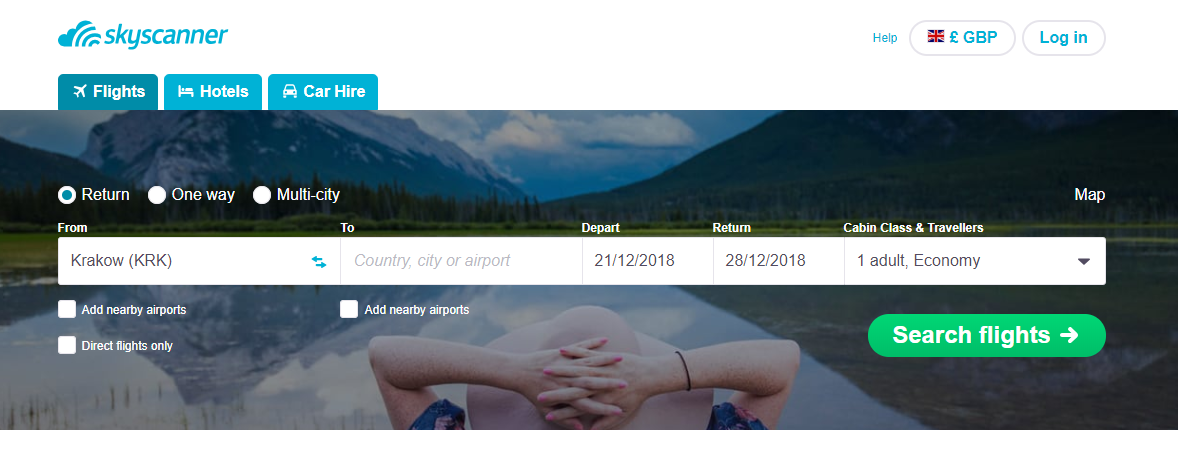
\includegraphics[scale=0.50, keepaspectratio]{skyscanner_main.png}
\caption{Panel wyszukiwania lotów aplikacji Skyscanner}
\label{fig:skyscanner_main}
\end{figure}


\newpage
\section{Wyszukiwarka lotów Google Flights}
text
\newpage
\section{Porównanie aplikacji}
text
\newpage

\chapter{Projekt aplikacji}
test
\newpage

\begin{thebibliography}{9}
\bibitem{xml}
XML. Almanach, Elliotte Rusty Harold, W.Scott Means, Wydawnictwo O'REILLY

\bibitem{json}
  \url{https://www.json.org/} \\
  Stan na dzień 03.01.2019

\bibitem{html}
	\url{https://en.wikipedia.org/wiki/HTML} \\
	Stan na dzień 04.01.2019
\bibitem{ehcache}
Instant Effective Caching with Ehcache, Daniel Wind, Packt Publishing
\end{thebibliography}



\end{document}